\section{Main Rotor}

\begin{tabularx}{\textwidth}{ | L | c | c | }
  \hline
  \textbf{Parameter}                    & \textbf{Value}   & \textbf{Reference} \\ \hline
  \endfirsthead
  \hline
  \textbf{Parameter}                    & \textbf{Value}   & \textbf{Reference} \\ \hline
  \endhead
  Main rotor diameter                   & 16.36 m          & \cite{Janes20042005,UH60_OperatorsManual} \\ \hline
  Main rotor number of blades           & 4                & \cite{NASA-CR-166309} \\ \hline
  Main rotor blade chord                & 0.53 m           & \cite{Janes20042005,NASA-CR-166309} \\ \hline
  Main rotor blade airfoil              & SC1095/SC1094 R8 & \cite{NASA-CR-166309,NASA-TP-2003-212265} \\ \hline
  Main rotor solidity                   & 0.0826           & \cite{NASA-CR-166309} \\ \hline
  Main rotor total blades area          & 17.36 m\textsuperscript{2} & \cite{NASA-CR-166309} \\ \hline
  Main rotor blade tip sweep            & 20.0\degree      & \cite{NASA-CR-166309} \\ \hline
  Main rotor blade twist                & -18.0\degree     & \cite{NASA-CR-166309} \\ \hline
  Main rotor shaft inclination angle    & 3.0\degree       & \cite{NASA-CR-166309} \\ \hline
  Main rotor nominal rotation speed     & 27 rad/s (258 rpm) & \cite{NASA-CR-166309} \\ \hline
  Main rotor hinge offset               & 0.38 m           & \cite{NASA-CR-166309} \\ \hline
  Main rotor blade spar lenght          & 1.17 m           & \cite{NASA-CR-166309} \\ \hline
  Main rotor blade tip lift loss factor & 0.97             & \cite{NASA-CR-166309} \\ \hline
  Main rotor blade section lift curve slope & 5.73 rad\textsuperscript{-1} & \cite{NASA-TM-85890} \\ \hline
  Main rotor maximum thrust coefficient & 0.1846           & \cite{NASA-TM-85890} \\ \hline
  Main rotor single blade weight        & 116.53 kg        & \cite{NASA-CR-166309} \\ \hline
  Main rotor single blade first moment of mass & 385.66 kg$\cdot$m & \cite{NASA-CR-166309} \\ \hline
  Main rotor single blade moment of inertia about flapping hinge & 2~050.81 kg$\cdot$m\textsuperscript{2} & \cite{NASA-CR-166309} \\ \hline
  Main rotor hub stationline            & 8.67 m           & \cite{UH60_MaintenanceManual} \\ \hline
  Main rotor hub waterline              & 8.00 m           & \cite{UH60_MaintenanceManual} \\ \hline
  \caption{Main rotor data}
\end{tabularx}

\begin{figure}[h!]
  \centering
  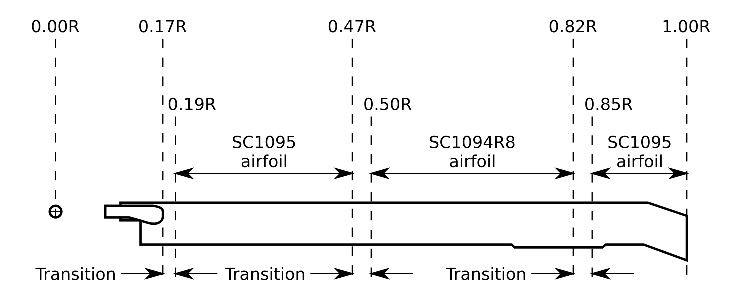
\includegraphics[width=120mm]{eps/uh60_blade.eps}
  \caption{Main rotor blade airfoil section locations \cite{NASA-TM-103985}}
\end{figure}

%%%%%%%%%%%%%%%%%%%%%%%%%%%%%%%%%%%%%%%%%%%%%%%%%%%%%%%%%%%%%%%%%%%%%%%%%%%%%%%%

\clearpage
\subsection{Symbols}

\begin{tabularx}{\textwidth}{ L l l l }
  \hline
  \textbf{Symbol} & \textbf{Mnemonic} & \textbf{Unit} & \textbf{Description} \\ \hline
  \endfirsthead
  \hline
  \textbf{Symbol} & \textbf{Mnemonic} & \textbf{Unit} & \textbf{Description} \\ \hline
  \endhead
  $A_{A0F}$ & A0FMR & deg & Steady flapping (coning) \\
  $A_{A1F}$ & A1FMR & deg & Longitudinal first harmonic flapping \\
  $B_{B1F}$ & B1FMR & deg & Lateral first harmonic flapping \\
  & & & \\
  ${\alpha}_{TRANS}$ & AFTFMR & deg & Transformed angle of attack for map entry \\
  $C_{LY}$           & CLMR   & -   & Blade segment lift coefficient \\
  $C_{DY}$           & CDMR   & -   & Blade segment drag coefficient \\
  $BTLMR$            & BTLMR  & -   & Blade tip lift loss factor \\
  ${\dot L}_{DT}$    & LD.MR  & m/s & Axial rate of lag damper \\
  $F_{\delta}$       & FLD.MR & N   & Axial force output from lag damper \\
  \caption{Main rotor symbols}
\end{tabularx}

%%%%%%%%%%%%%%%%%%%%%%%%%%%%%%%%%%%%%%%%%%%%%%%%%%%%%%%%%%%%%%%%%%%%%%%%%%%%%%%%

\clearpage
\subsection{Airfoils Ordinates}

\subsubsection{SC1094 R8}

\begin{figure}[h!]
  \centering
  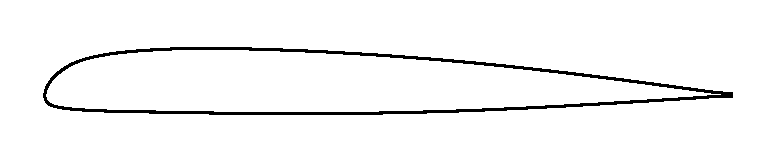
\includegraphics[width=127mm]{eps/airfoil_SC1094R8.eps}
  \caption{SC1094 R8}
\end{figure}

\csvreader[
  no head,
  longtable=cccc,
  table head=
    \toprule
    \multicolumn{2}{c}{\bfseries Upper surface} & \multicolumn{2}{c}{\bfseries Lower surface} \\
    x/c & y/c & x/c & y/c \\ \midrule
    \endfirsthead
    \multicolumn{2}{c}{\bfseries Upper surface} & \multicolumn{2}{c}{\bfseries Lower surface} \\
    x/c & y/c & x/c & y/c \\ \midrule
    \endhead,
  before first line={},
  late after line=\\,
  late after last line=\\ \bottomrule \caption{SC1094 R8 \cite{NASA-TP-2003-212265}},
  before reading={},
  after reading={}
]
{csv/airfoil_SC1094R8.csv}
{1=\colxu,2=\colyu,3=\colxl,4=\colyl}
{\colxu & \colyu & \colxl & \colyl}

\subsubsection{SC1095}

\begin{figure}[h!]
  \centering
  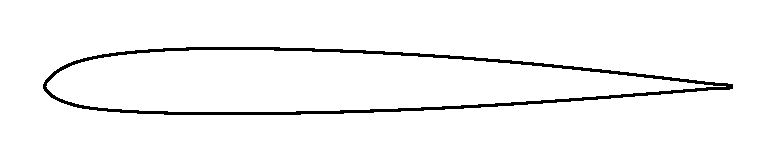
\includegraphics[width=127mm]{eps/airfoil_SC1095.eps}
  \caption{SC1095}
\end{figure}

\csvreader[
  no head,
  longtable=cccc,
  table head=
    \toprule
    \multicolumn{2}{c}{\bfseries Upper surface} & \multicolumn{2}{c}{\bfseries Lower surface} \\
    x/c & y/c & x/c & y/c \\ \midrule
    \endfirsthead
    \multicolumn{2}{c}{\bfseries Upper surface} & \multicolumn{2}{c}{\bfseries Lower surface} \\
    x/c & y/c & x/c & y/c \\ \midrule
    \endhead,
  before first line={},
  late after line=\\,
  late after last line=\\ \bottomrule \caption{SC1095 \cite{NASA-TP-2003-212265}},
  before reading={},
  after reading={}
]
{csv/airfoil_SC1095.csv}
{1=\colxu,2=\colyu,3=\colxl,4=\colyl}
{\colxu & \colyu & \colxl & \colyl}

%%%%%%%%%%%%%%%%%%%%%%%%%%%%%%%%%%%%%%%%%%%%%%%%%%%%%%%%%%%%%%%%%%%%%%%%%%%%%%%%

\clearpage
\subsection{Blade Twist}

\csvreader[
  no head,
  longtable=cc,
  table head=
    \toprule
    XSEGMR & TWSTMR \\ 
    {[-]} & {[deg]} \\ \midrule
    \endfirsthead
    XSEGMR & TWSTMR \\ 
    {[-]} & {[deg]} \\ \midrule
    \endhead,
  before first line={},
  late after line=\\,
  late after last line=\\ \bottomrule \caption{Main rotor blade twist \cite{NASA-CR-166309}},
  before reading={},
  after reading={}
]
{csv/uh60_main_rotor_twstmr.csv}
{1=\colyr,2=\coltwist}
{\colyr & \coltwist}

\begin{figure}[ph!]
  \centering
  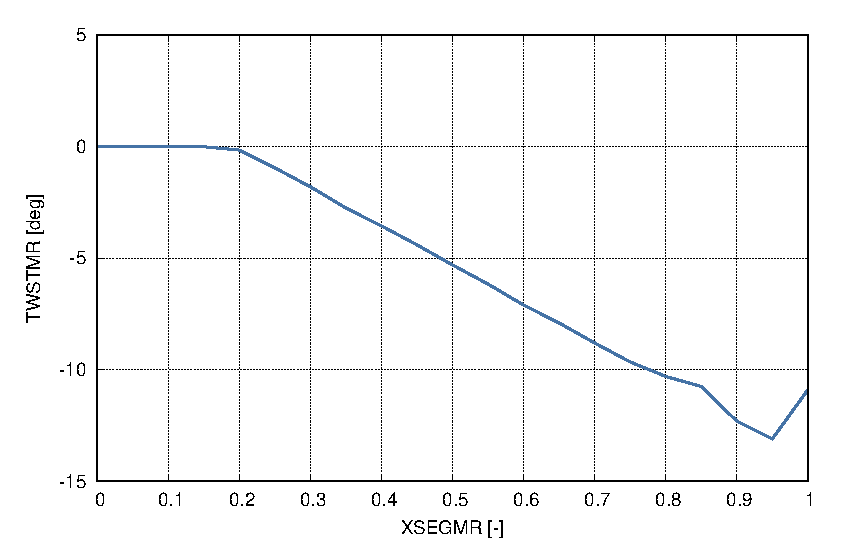
\includegraphics[width=140mm]{eps/uh60_main_rotor_twstmr.eps}
  \caption{Main rotor blade twist \cite{NASA-CR-166309}}
\end{figure}

%%%%%%%%%%%%%%%%%%%%%%%%%%%%%%%%%%%%%%%%%%%%%%%%%%%%%%%%%%%%%%%%%%%%%%%%%%%%%%%%

\clearpage
\subsection{Blade Section Aerodynamic Characteristics}

\csvreader[
  no head,
  longtable=ccc,
  table head=
    \toprule
    $\alpha_{TRANS}$ & $C_{LY}$ & $C_{DY}$ \\ 
    {[deg]} & {[-]} & {[-]} \\ \midrule
    \endfirsthead
    $\alpha_{TRANS}$ & $C_{LY}$ & $C_{DY}$ \\ 
    {[deg]} & {[-]} & {[-]} \\ \midrule
    \endhead,
  before first line={},
  late after line=\\,
  late after last line=\\ \bottomrule \caption{SC1095 aerodynamic coefficients \cite{NASA-CR-166309}},
  before reading={},
  after reading={}
]
{csv/SC1095_CR-166309.csv}
{1=\colaoa,2=\colcz,3=\colcx}
{\colaoa & \colcz & \colcx}

\begin{figure}[p]
  \centering
  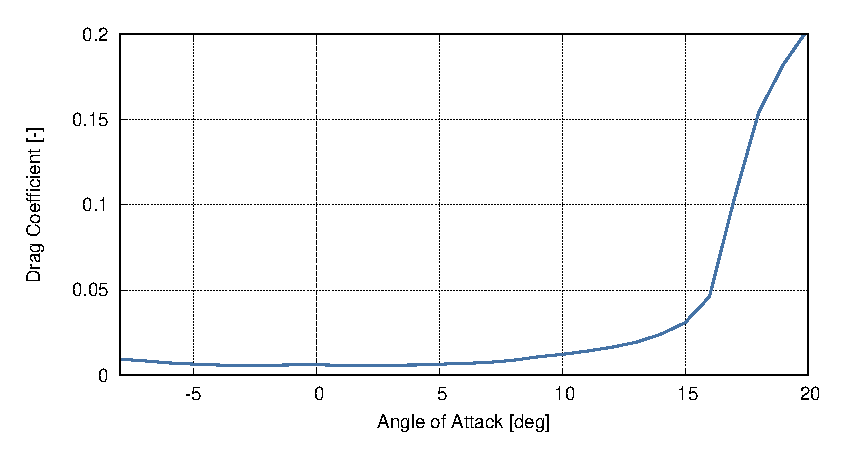
\includegraphics[width=140mm]{eps/uh60_blade_sc1095_cx.eps}
  \caption{SC1095 drag coefficient \cite{NASA-CR-166309}}
\end{figure}

\begin{figure}[p]
  \centering
  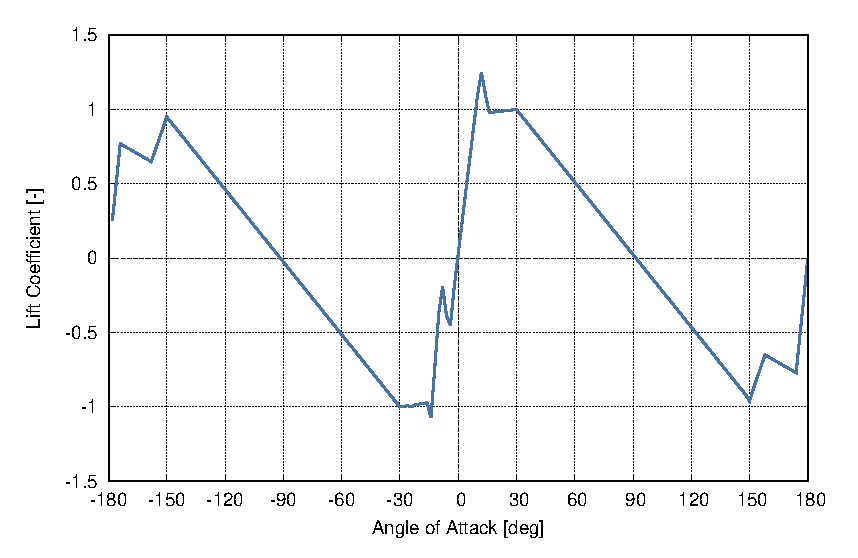
\includegraphics[width=140mm]{eps/uh60_blade_sc1095_cz.eps}
  \caption{SC1095 lift coefficient \cite{NASA-CR-166309}}
\end{figure}

\clearpage
\newgeometry{margin=1cm}
\thispagestyle{empty}
\begin{sidewaystable}
  \begin{center}
    \scalebox{0.9}
    {
      \begin{tabular}{ c c c c c c c c c c c c }
        \toprule
        $\alpha_{TRANS}$ & \multicolumn{11}{c}{$C_{LY}$} \\
        {[deg]} & Ma=0.0 & Ma=0.1 & Ma=0.2 & Ma=0.3 & Ma=0.4 & Ma=0.5 & Ma=0.6 & Ma=0.7 & Ma=0.8 & Ma=0.9 & Ma=10.0 \\ \midrule
        \csvreader[
          column count=12,
          no head,
          late after line=\\
        ]
        {csv/SC1095_CR-166309_cz.csv}
        {}
        {\csvlinetotablerow}
        \bottomrule
      \end{tabular}
    }
    \caption{SC1095 lift coefficient \cite{NASA-CR-166309}}
  \end{center}
\end{sidewaystable}
\restoregeometry

\clearpage
\newgeometry{margin=1cm}
\thispagestyle{empty}
\begin{sidewaystable}
  \begin{center}
    \scalebox{0.9}
    {
      \begin{tabular}{ c c c c c c c c c c c c }
        \toprule
        $\alpha_{TRANS}$ & \multicolumn{11}{c}{$C_{DY}$} \\
        {[deg]} & Ma=0.0 & Ma=0.1 & Ma=0.2 & Ma=0.3 & Ma=0.4 & Ma=0.5 & Ma=0.6 & Ma=0.7 & Ma=0.8 & Ma=0.9 & Ma=10.0 \\ \midrule
        \csvreader[
          column count=12,
          no head,
          late after line=\\
        ]
        {csv/SC1095_CR-166309_cx.csv}
        {}
        {\csvlinetotablerow}
        \bottomrule
      \end{tabular}
    }
    \caption{SC1095 drag coefficient \cite{NASA-CR-166309}}
  \end{center}
\end{sidewaystable}
\restoregeometry

\begin{figure}[p]
  \centering
  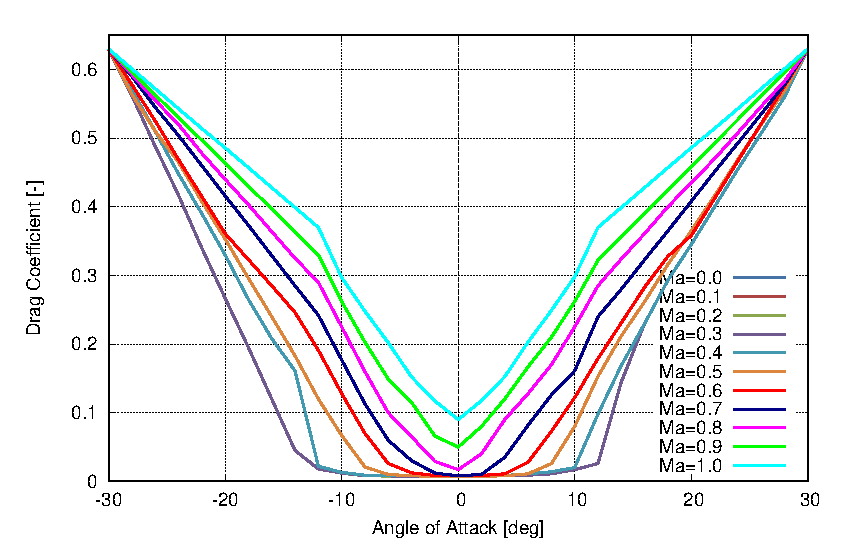
\includegraphics[width=140mm]{eps/uh60_blade_sc1095_cx_2.eps}
  \caption{SC1095 drag coefficient \cite{NASA-CR-166309}}
\end{figure}

\begin{figure}[p]
  \centering
  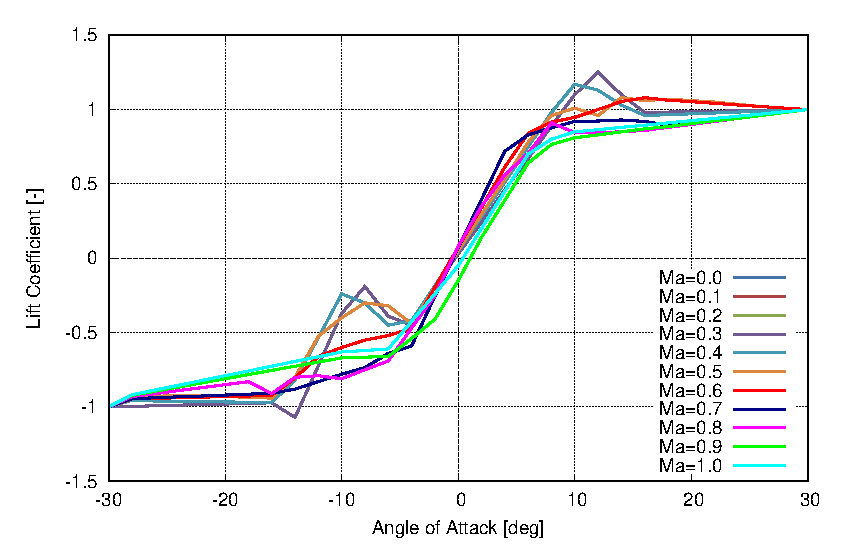
\includegraphics[width=140mm]{eps/uh60_blade_sc1095_cz_2.eps}
  \caption{SC1095 lift coefficient \cite{NASA-CR-166309}}
\end{figure}

%%%%%%%%%%%%%%%%%%%%%%%%%%%%%%%%%%%%%%%%%%%%%%%%%%%%%%%%%%%%%%%%%%%%%%%%%%%%%%%%

\clearpage
\subsection{Lag Damper Force Characteristics}

\csvreader[
  no head,
  longtable=cc,
  table head=
    \toprule
    ${\dot L}_{DT}$ & $F_{\delta}$ \\ 
    {[m/s]} & {[N]} \\ \midrule
    \endfirsthead
    ${\dot L}_{DT}$ & $F_{\delta}$ \\ 
    {[m/s]} & {[N]} \\ \midrule
    \endhead,
  before first line={},
  late after line=\\,
  late after last line=\\ \bottomrule \caption{Lag damper force \cite{NASA-CR-166309}},
  before reading={},
  after reading={}
]
{csv/uh60_main_rotor_fldmr.csv}
{1=\colyr,2=\coltwist}
{\colyr & \coltwist}

\begin{figure}[ph!]
  \centering
  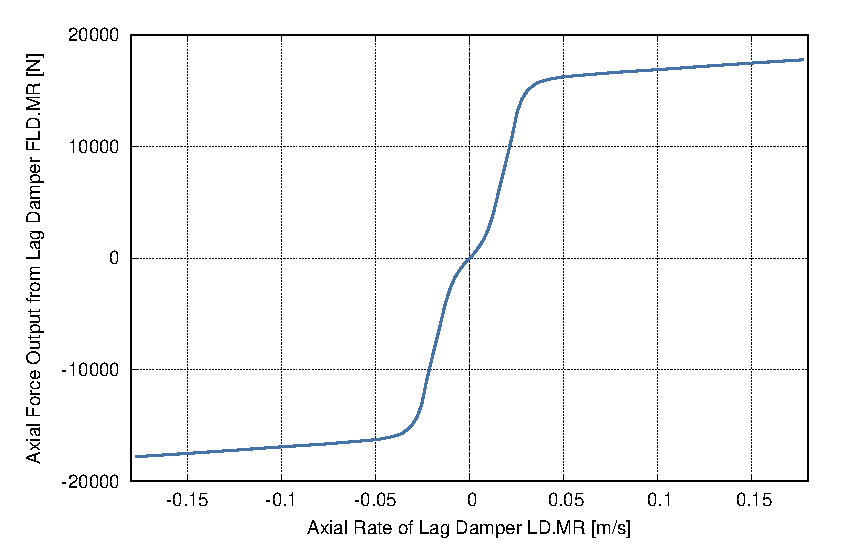
\includegraphics[width=140mm]{eps/uh60_main_rotor_fldmr.eps}
  \caption{Lag damper force \cite{NASA-CR-166309}}
\end{figure}
